% --------------------------------------------------------------
% This is all preamble stuff that you don't have to worry about.
% Head down to where it says "Start here"
% --------------------------------------------------------------
 
\documentclass[12pt]{article}
 
\usepackage[margin=1in]{geometry} 
\usepackage{amsmath,amsthm,amssymb}
\usepackage{gensymb}
\usepackage{graphicx}
 \usepackage{tikz,pgfplots}
\usepackage{float}
\usepackage{enumitem}
\usepackage[utf8]{inputenc}


\newcommand{\N}{\mathbb{N}}
\newcommand{\Z}{\mathbb{Z}}

\newcommand{\slantedgrid}[4]{%
   \pgfmathtruncatemacro{\result}{#1+#3}
   \foreach \x in {#1,...,\result} \draw (\x,#2) -- ++(#4,#4);%
   \pgfmathtruncatemacro{\result}{#2+#4}
   \foreach \y in {#2,...,\result} \draw (#1+\y-#2,\y) -- ++(#3,0);%
 }
 \newcommand{\specialcell}[2][c]{%
  \begin{tabular}[#1]{@{}c@{}}#2\end{tabular}}
  
\DeclareMathOperator\erf{erf}
 
\newenvironment{theorem}[2][Theorem]{\begin{trivlist}
\item[\hskip \labelsep {\bfseries #1}\hskip \labelsep {\bfseries #2.}]}{\end{trivlist}}
\newenvironment{lemma}[2][Lemma]{\begin{trivlist}
\item[\hskip \labelsep {\bfseries #1}\hskip \labelsep {\bfseries #2.}]}{\end{trivlist}}
\newenvironment{exercise}[2][Exercise]{\begin{trivlist}
\item[\hskip \labelsep {\bfseries #1}\hskip \labelsep {\bfseries #2.}]}{\end{trivlist}}
\newenvironment{problem}[2][Problem]{\begin{trivlist}
\item[\hskip \labelsep {\bfseries #1}\hskip \labelsep {\bfseries #2.}]}{\end{trivlist}}
\newenvironment{question}[2][Question]{\begin{trivlist}
\item[\hskip \labelsep {\bfseries #1}\hskip \labelsep {\bfseries #2.}]}{\end{trivlist}}
\newenvironment{corollary}[2][Corollary]{\begin{trivlist}
\item[\hskip \labelsep {\bfseries #1}\hskip \labelsep {\bfseries #2.}]}{\end{trivlist}}
 
\begin{document}
\providecommand{\e}[1]{\ensuremath{\times 10^{#1}}}
\providecommand{\ex}[1]{\ensuremath{10^{#1}}}
% --------------------------------------------------------------
%                         Start here
% --------------------------------------------------------------
 
\title{HW 9}
\author{Levon Dovlatyan \\ SI: 24451582\\ E45} 
\date{Nov 21, 2014}
\maketitle
 
\begin{problem}{12.10} 
If the polymer evaluated in Problem 12.9 is polypropylene, what would be the \textbf{(a)} coiled length and \textbf{(b)} extended length of the average molecule?

\begin{figure}[H]
\centering
\begin{tabular}{c | c | c}
n Range & $n_i$ (Mid Value) & Population fraction \\ \hline
1-100 & 50 & -- \\ \hline
101-200 & 150 & -- \\ \hline
201-300 & 250 & 0.01 \\ \hline
301-400 & 350 & 0.10 \\ \hline
401-500 & 450 & 0.21 \\ \hline
501-600 & 550 & 0.22 \\ \hline
601-700 & 650 & 0.18 \\ \hline
701-800 & 750 & 0.12 \\ \hline
801-900 & 850 & 0.07 \\ \hline
901-1000 & 950 & 0.05 \\ \hline
1001-1100 & 1050 & 0.02 \\ \hline
1101-1200 & 1150 & 0.01 \\ \hline
1201-1300 & 1250 & 0.01 \\ \hline
\end{tabular}
\caption{table from problem 12.9}
\end{figure}
\end{problem}

\textbf{(a)} In order to calculated $L = l\sqrt{m}$ where $m = 2n$ and $l$ is the length of a single bond, we need the degree of polymerization from table 1 above. We can get this by multiplying the percent fraction (column 3) by the Mid values (column 2) and sum them up.

\begin{figure}[H]
\begin{tabular}{c | c | c | c | c | c | c | c | c | c | c | c}
average n value (a.u)&2.5 &35 &94.5 &121 &117 &90 &59.5 &47.5 & 21 &11.5 &12.5 \\ \hline
\end{tabular}
\end{figure}
The sum of these values is $n = 612$. Now to get the length of a single bond, we can simple find the radius of a carbon atom and multiply by 2. This is assuming that each mer is touching the mer adjacent to it. The radius of carbon here is 0.077 nm [1].
\begin{align*}
L = l\sqrt{m} = l\sqrt{2n} = 2*0.077\,nm\sqrt{2(612)} = 5.39\,nm
\end{align*}

\textbf{(b)} We know that carbon tends to bond in a tetrahedral form with angles of 109.5$\degree$. In order to get an uncoiled length, we use equation 12.5 [1] in the textbook.
\begin{align*}
L_{ext} = ml\sin{(109.5\degree/2)} = 2*0.077*2*612sin{(109.5/2)} = 154\, nm
\end{align*}

\begin{problem}{12.21}
In Problem 11.5, the mass reduction in an automobile design was calculated based on trends in metal alloy selection. A more complete picture is obtained by noting that, in the same 1975 to 1985 period, the volume of polymers used increased from 0.064 $m^3$ to 0.100 $m^3$. Estimate the mass reduction (compared to 1975) including this additional polymer data. (Approximate the polymer density as Th$\text{O}_2$)
\end{problem}

\begin{problem}{ref (11.5)}
Between 1975 and 1985, the volume of all iron and steel in a given automobile model decreased from 0.162 $\text{m}^3)$ to 0.116 $\text{m}^3)$. In the same time frame, the volume of all aluminum alloys increased from 0.012 $\text{m}^3)$ to 0.023 $\text{m}^3)$. Using the densities of pure Fe and Al, estimate the mass reduction resulting from this trend in materials substitution.
\end{problem}

From appendix 1 [1], the density of Fe is 7.87 g/$\text{cm}^3$ and for Al 2.70 g/$\text{cm}^3$. \\

We use this information to find the mass resulting in the difference of volume.

\begin{align*}
m_{\text{Fe}} =& \rho V = 7.87 \,\text{g}/\text{cm}^3 * 10^6 \,\text{cm}^3 * (0.162-0.116) * \frac{1}{10^3 \,\text{kg}} = 362.02 \,\text{kg} \\
m_{\text{Al}} =& \rho V = 2.70 \,\text{g}/\text{cm}^3 * 10^6 \,\text{cm}^3 * (0.023-0.012) * \frac{1}{10^3 \,\text{kg}} = 29.7 \,\text{kg} \\
m_{\text{Poly}} =& \rho V = 1 \,\text{Mg}/\text{cm}^3 * 10^6 \,\text{cm}^3 * (0.100-0.064) * 10^3 \,\text{kg} = 36 \,\text{kg}
\end{align*}

Now for the mass reduction we have $362.02 - 29.7 - 36 = 296.32$ kg mass reduction.

\begin{problem}{12.31}
Calculate the average separation distance between the centers of adjacent glass spheres in the nylon described in Problem 12.30. (Assume a simple cubic array of dispersed particles as in Problem 11.20).
\end{problem}

\begin{problem}{ref 12.30}
Some injection moldable nylon 66 contains 40 wt\% glass spheres as a filler.  Improved mechanical properties are the result.  If the average glass sphere diameter is 100 $\mu$m, estimate the density of such particles per cubic millimeter.  
\end{problem}

According to Ex 2.5 [1], the density of nylon 66 is $\rho_n = 1140$ kg/$\text{m}^3$ and for glass $\rho_g = 2540$ kg/$\text{m}^3$. We assume a total mass of 1kg which means we have 0.4kg glass and 0.6kg nylon.

\begin{align*}
V_{tot} = V_n + V_g = \frac{m_n}{\rho_n} + \frac{m_g}{\rho_g} = \frac{0.6\,\text{kg}}{1140 \text{kg}/\text{m}^3} + \frac{0.4\,\text{kg}}{2540 \text{kg}/\text{m}^3} \approx 6.838\e{-4} \,\text{m}^3
\end{align*}

Next we want the \# of glass spheres in a Volume of glass, (Note radius of glass sphere is 50 microns)

\begin{align*}
\frac{V_g}{V_{g-spheres}} = \frac{1.575\e{-4}}{(4\pi/3)(50\e{-6})^3} \approx 3\e{8} \,\text{glass spheres in a volume of glass}
\end{align*}

Now we want the \# of glass spheres per a unit of total volume,

\begin{align*}
\frac{\text{\# of glass spheres}}{V_{tot}} = \frac{3\e{8} \,\text{spheres}}{6.838\e{-4}\,\text{m}^3} \approx 4.39 \e{11} \,\text{\# spheres / total volume}
\end{align*}

Now in order to make sure we have units of meters and not inverse meters cubed we take the cube root and inverse of the above number,

\begin{align*}
(\sqrt[3]{4.39\e{11}})^{-1} = 1.316\e{-4} \approx 0.132 \,\text{mm}
\end{align*}

\begin{problem}{12.47}
 On a plot similar to that displayed in Figure 12.17, show the composite modulus for (a) 60 vol\% fibers (the result of Example 12.8) and (b) 50 vol\% fibers (the result of Practice Problem 12.8).  Include the individual glass and polymer plots.
\end{problem}

Refer to the plot below.
\begin{figure}[H]
\centering
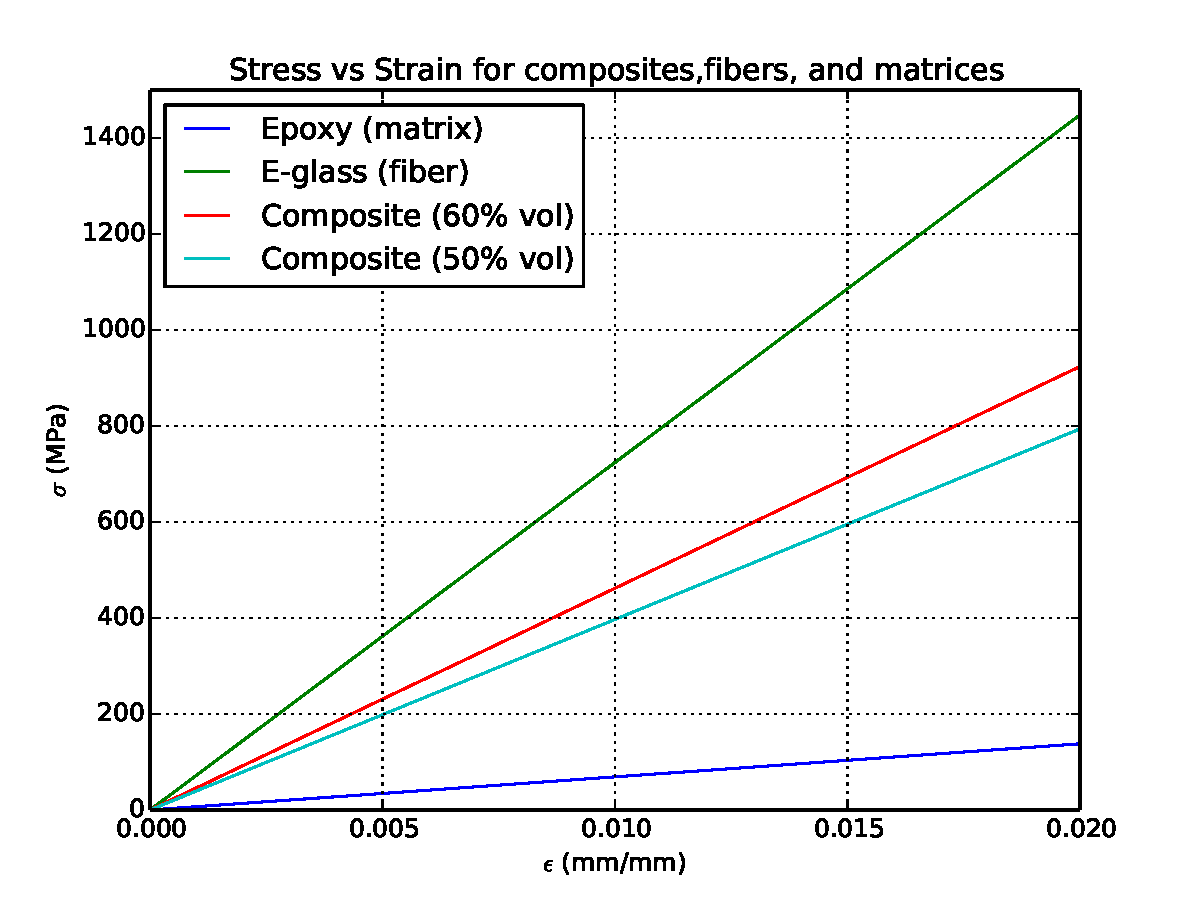
\includegraphics[width=350pt]{1247plot.pdf}
\caption{The slopes used are: $72.4\e{3}$MPa for E-glass, $6.9\e{3}$MPa for Epoxy, $46.2\e{3}$MPa for 60\% Composite, and $39.7\e{3}$MPa for 50\% Composite.}
\end{figure}

\begin{problem}{12.62}
n Problem 6.9, a competition among various metallic pressure-vessel materials was illustrated.  We can expand the selection process by including some composites, as listed in the following table: 
\begin{figure}[H]
\centering
\begin{tabular}{c | c | c | c | c | c}
Materials & $\rho$(Mg/$\text{m}^3$) & \specialcell{Cost \\ (\$/kg)} & Y.S. (MPa) & \specialcell{$\rho$/Y.S. \\(Mg*MPa/$\text{m}^3$)} & \specialcell{$\rho$*Cost/Y.S. \\ ((\$Mg*MPa/$\text{m}^3$))}\\ \hline
1040 carbon Steel & 7.80 & 0.63 & -- &  -- & --\\ \hline
304 stainless steel & 7.80 & 3.70 & -- &  -- & --\\ \hline
3003-H14 aluminum & 2.73 & 3.00 & -- & -- & --\\ \hline
Ti-5Al-2.5Sn & 4.46 & 15.00 & -- & -- & -- \\ \hline
Reinforced concrete & 2.50 & 0.40 & 200 & .0125 & .005 \\ \hline
Fiberglass & 1.80 & 3.30 & 200 & .009 & .0297 \\ \hline
C fiber-reinforced polymer & 1.50 & 70.00 & 600 & .0025 & .175 \\ \hline
\end{tabular}
\caption{Material cost,yield strength, and density}
\end{figure}
\textbf{(a)} From this expanded list, select the material that will produce the lightest vessel. \textbf{(b)} Select the materials that will produce the minimum-cost vessel.  
\end{problem}

\textbf{(a)} Looking at problem 6.9 [1], we see that the mass of the lightest vessel is $m = C\frac{\rho}{Y.S.}$ where C in this case is some arbitrary constant. So in order to minimize mass, we look for the smalles value of the ratio $\frac{\rho}{Y.S.}$. Looking at figure 3, column 5, we see that \textbf{carbon fiber-reinforced polymer} has the smallest value. \\

\textbf{(b)} Now in order to also minimize cost, we can simply multiply the cost by our ratio we calculated in part a. The idea is that if you want to minimize two variables, you know that their product must also be minimized. So we can multiply the costs by the ratio we calculated in part a. The last column in figure 3 contains this product. The smallest value in this case is 0.005 which corresponds to \textbf{reinforced concrete}.
\section{References}
\begin{enumerate}
\item James F. Shackelford, Introduction to Materials Science for Engineers, Seventh Edition, Pearson Higher Education, Inc., Upper Saddle River, New Jersey (2009).
\end{enumerate}




% --------------------------------------------------------------
%     You don't have to mess with anything below this line.
% --------------------------------------------------------------
 
\end{document}
